\chapter{\IfLanguageName{dutch}{Stand van zaken}{State of the art}}
\label{ch:stand-van-zaken}

% Tip: Begin elk hoofdstuk met een paragraaf inleiding die beschrijft hoe
% dit hoofdstuk past binnen het geheel van de bachelorproef. Geef in het
% bijzonder aan wat de link is met het vorige en volgende hoofdstuk.

% Pas na deze inleidende paragraaf komt de eerste sectiehoofding.

%Dit hoofdstuk bevat je literatuurstudie. De inhoud gaat verder op de inleiding, maar zal het onderwerp %van de bachelorproef *diepgaand* uitspitten. De bedoeling is dat de lezer na lezing van dit hoofdstuk %helemaal op de hoogte is van de huidige stand van zaken (state-of-the-art) in het onderzoeksdomein. %Iemand die niet vertrouwd is met het onderwerp, weet nu voldoende om de rest van het verhaal te %kunnen volgen, zonder dat die er nog andere informatie moet over opzoeken.

%Je verwijst bij elke bewering die je doet, vakterm die je introduceert, enz. naar je bronnen. In \LaTeX{} %kan dat met het commando \texttt{$\backslash${textcite\{\}}} of \texttt{$\backslash${autocite\{\}}}. Als %argument van het commando geef je de ``sleutel'' van een ``record'' in een bibliografische databank %in het Bib\LaTeX{}-formaat (een tekstbestand). Als je expliciet naar de auteur verwijst in de zin, gebruik %je \texttt{$\backslash${}textcite\{\}}.
%Soms wil je de auteur niet expliciet vernoemen, dan gebruik je \texttt{$\backslash${}autocite\{\}}. In de %volgende paragraaf een voorbeeld van elk.

\section{Technology Stack}
\label{sec:techstack}
Where the legacy tech stack centered around JavaScript for front-end and PHP for back-end development, the programming language of preference for all recent and new development is TypeScript. When it comes to the web application framework of preference, Showpad standerdises on  Angular.  
\subsection{TypeScript}
TypeScript is a JavaScript-based programming language developed by Microsoft and first released in October 2012 under Apache 2.0 license. Typescript is a superset of JavaScript with the addition of static type checking as its primary differentiator. TypeScript applies to both front-end and back-end development. The cross-stack applicability of this programming language is a crucial differentiator and why many web application companies select TypeScript as the dominant language of preference. 
\subsection{Angular}
Angular is a TypeScript-based web application framework. Angular is the successor to AngularJS developed from the ground up at Google and first officially released in 2016 . Angular is written in TypeScript, and open-sourced under an MIT license. Angular has a cadence of up to 2 major releases per year, with a Long Time Support window of 18 months. The latest major release is version 14 and has been available since early June 2022.

An Angular application comprises Angular Components, organized in NgModules, which are collections of functional sets of related code.

All applications have at least a root module for bootstrapping and several feature modules to structure the application's features. Components define Views and use Services, which comprise the UI building blocks and functionality. Modules, Components, and Services are classes that use Decorators to provide metadata on how to use them. The Angular Router service provides sophisticated navigation capabilities.
\subsection{Redux}
Redux is a "predictable state container" for JavaScript applications. It is both a pattern and a library for implementing complex state management at scale. It was created at Facebook by Dan Abramov \& Andrew Clark in 2015. Facebook's Fluxclient-side web applications architecture forms the inspiration for Redux. 

Redux has three main principles: "Single source of truth", "State is read-only," and "Changes are made with pure functions".
\subsubsection{Single source of truth}
The application's global state resides in an object tree within a single store.
Because the state from the server can be serialized and hydrated into the client without additional coding work, this makes it simple to design universal apps. A single state tree also facilitates speedier development cycles by allowing you to persist your app's state during development and makes it simpler to debug and inspect an application. Saving state in a single tree is a viable option to simplify the implementation of historically challenging functionality like undo/redo.
\subsubsection{State is read-only}
The only way to change the state is to emit an action, an object describing what happened.
Doing this guarantees that neither network callbacks nor views will write directly to the state. Instead, they express an intent to transform the state. There are no undetectable subtle race conditions because everything is centralized and implemented in tight order. Actions may be logged, serialized, stored, and then replayed for testing or debugging since they are just plain objects.
\subsubsection{Changes are made with pure functions}
To specify how actions transform the state tree, you write pure reducers.
Reducers are pure functions that take a state and an action as inputs and output the new state. Never modify the initial state; always return new state objects. You can start with a single reducer and divide it into smaller reducers that control particular aspects of the state tree as your project develops. Reducers are functions, so you may customize their calling order, pass extra data, or even create reusable reducers for frequent tasks like pagination.
With these three principles in place, a clear pattern is present, as shown in the following image.
\subsection{RxJS}
According to RxJS home page, RxJS is a library for reactive programming using Observables, to make it easier to compose asynchronous or callback-based code. This project is a rewrite of Reactive-Extensions/RxJS with better performance, better modularity, better debuggable call stacks, while staying mostly backward compatible, with some breaking changes that reduce the API surface
\subsection{NgRx}
NgRx, inspired by Redux, builds on RxJS and provides reactive state management specifically for Angular apps. It enables the management of local and global state across an Angular application. It serves to unify the events in the application facilitating cleaner component architecture and isolating side effects. 
\section{Design System}
\label{sec:designsystem}
In large-scale digital products like enterprise web applications, the challenge of getting and keeping a consistent and coherent product design is non-trivial. Multiple teams and designers working on one product suite can create a patchwork of styles and component implementations. To resolve this issue, companies develop a design system. A design system is a library of reusable components, patterns, style guides, and best practices constrained by design standards. The design team owns the design system, but the development and maintenance are a joint responsibility of both designers and application developers. Next to the coherence and consistency of the User Experience (UX) and User Interface (UI), a design system also provides a productivity boost for the product development team, as design components are reused with every new functionality added to the product.
\section{Repository Management}
Two dominant models for structuring code bases exist in the version control space. \gls{Monorepo} and Polyrepo. 

In a \gls{Monorepo} setup, the codebases of the multiple projects are kept together in a single repository. These projects have a well-defined relationship. The colocation of code and the well-defined relationship among the projects make a Monorepo a Monorepo.

In a Polyrepo setup, repositories are created per project or team, typically resulting in a single build artifact and build pipeline.

For the development of the front-end stack, Showpad chose the \gls{Monorepo} model for the following reasons:
\begin{itemize}
    \item The simplicity of the model
    \item The ease of code reuse
    \item Simplified dependency management
    \item cross-team code modifications
\end{itemize}

This \gls{Monorepo} model, as implemented today, does come with its drawbacks. Especially the queueing of work in front of the CI/CD pipeline, as its \gls{Cycletime} grows with the codebase's size and dependencies.
\section{Deployment Architecture}
\label{sec:deploymentarchitecture}
In software deployment architecture, a modularity scale applies when evaluating an application's core architectural structure. The two extremes on that scale are a Monolith architecture and a Micro-Services architecture.
\subsection{Monolith Architecture}
A monolith architecture is the simplest form of deployment architecture. The application and all it's functionality is compiled into a single executable and deployed accordingly. 

Monolithic software is intended to be self-contained, with firmly tied rather than loosely related components or functions, as opposed to modular software programs. For code to be executed or compiled and for software to run under a monolithic architecture, each component and all of its related components must be present.

Single-tiered monolithic applications integrate several components into a single, substantial application. They frequently have enormous codebases as a result, which can be challenging to manage over time.

Additionally, if one part of the program needs to be updated, other parts might need to be rewritten as well, and the entire application needs to be recompiled and tested. Teams working on software development may not be as agile or quick due to the lengthy process. The method is still used despite these drawbacks since it has some benefits. Additionally, a lot of early apps were created as monolithic pieces of software; hence, the method cannot be entirely dismissed when those applications are still in use and need to be updated.

Many applications start as a monolith applications as its simplicity hase many advantages, especially in a development context were only a handful of developers are working on the product. As the codebase and functionality grows, and the number of developers involved scales, the monolith architecture loses its advantages.
\subsection{Microservices Architecture}
At the other end of the spectrum Microservices architecture, commonly referred to as so-called microservices, has generated a lot of attention in recent years. Software programs have gotten bigger and harder to administer, update, and maintain as they have gotten more complicated.

\Citeauthor*{Newman2015} is the reference author when it comes to thought leadership on Microservices. in his 2015 book titled ``Building Microservices, designing fine-grained systems'', he drove the microservices hype. The book starts from the advantages of the architectural concept, but spends equal attention to the drawbacks that it brings. It for sure does not paint a ``silver bullet'' picture on microservices.

In his 2020 book, ``Monolith to Microservices, Evolutionary patterns to transform your monolith'', \Citeauthor*{Newman2020}  builds on his inital narrative, and provides tips and tricks on how to evolve a monolith reality to a microservices architecture.

This issue is addressed by the relatively recent software development strategy known as microservices architecture, which divides complex software into separate deployable components or services. Large applications become more adaptable to change thanks to the separate deployment and management of these modular services.

The phrase "Micro-Web-Services" was initially used in 2005 by Resource Oriented Computing pioneer Peter Rodgers to describe the architectural style known as microservices. He was influential in outlining the fundamentals of a well-designed microservices platform to develop a more adaptable and service-oriented software architecture. A granular use of services was formed two years later by software architect Juval Löwy, who also sparked many expert-led case studies with encouraging results.

Microservices architecture is currently seen as the future of effective software development and maintenance and a hot topic.
Principles
\begin{itemize}
    \item Modeled around business domains
    \item Culture of automation
    \item Hide implementation details
    \item Decentralized governance
    \item Highly observable
    \item Isolate failure
    \item Deploy independently
\end{itemize}
These principles also apply to micro frontends in their way.
\subsection{Micro Frontends Architecture}
With the rise of more and more powerful browser and extended web application development frameworks, the Microservices philosophy invaded the frontend world. The reference book on the topic is \Citeauthor{Mezzalira2021}'s 2021 book ``Building Micro-Frontends, scaling teams and projects, empowering developers''. During my internship at Showpad I had the opportunity to join a video conference with Luca Mezzalira where we got invaluable tips on how to tackle micro frontends starting from today's Showpad reality.

Micro Frontends is an architectural approach to the frontend development with the same idea of microservices, splitting one extensive application or project into a collection of independent micro applications owned by different teams. 

Micro frontends aren’t a silver bullet, but it certainly has many advantages.
The main advantages of micro frontends are their scalability, the reusability of components, the ability to use different frameworks, more efficient development and deployment, and makes the applications easier to maintain, more stable, and easier to test.
\subsubsection{Scalability}
Micro frontends make it simple for us to scale a project. It enables the teams to expand their portion of the frontend with regular updates, which will cause the app to scale over time at a manageable rate with several teams each in charge of their own specific micro frontend implementations. It also allows to easily add new features and teams since a project built with micro frontends has a shell application that hosts all its “remote” applications.
\subsubsection{Different frameworks}
Since the concept of micro frontends is to have all kinds of micro applications work together as one extensive application, these micro applications can be implemented using different technology stacks and frameworks. Some teams might prefer React or Vue, and others might prefer Angular. Every team gets to pick and choose what framework they want to use.
\subsubsection{Maintenance and testing}
Because everything is divided into smaller parts, it is easier for teams to maintain and test their little portion of the project. No need to wait to spin up the entire application, just the part the team is working on.

But there are a couple of significant drawbacks. By breaking up the application into a multitude of smaller services, the complexity of the overall application structure increases substantially. So there is the potential to lose track of certain parts or risk a lack of communication. Another potential drawback is that the CI/CD pipeline needs substantial refactoring and automation with the micro frontend structure.

As mentioned before, most principles of microservices also apply to micro frontends, but here are the four main ones:
\begin{itemize}
    \item Business domain representation
    \item Autonomous codebase 
    \item Independent deployment
    \item Single-team ownership
\end{itemize}

To create a micro frontend environment, we have to decide on a couple of things:
\begin{itemize}
    \item Defining what a micro frontend is in your architecture
    \item Composing micro frontends
    \item Routing micro frontends
    \item Communication between micro frontends
\end{itemize}
To work out a successful micro frontend structure we have to ask ourselves a couple of essential yet challenging questions, mainly being:
\begin{itemize}
    \item How to communicate between micro frontends?
    \item How to route the user from one view to another?
    \item How to identify the size of a micro frontend?
\end{itemize}
\subsubsection{Two approaches to scope microfrontends}
There are two approaches to take when it comes to scoping our micro frontend applications, a horizontal split or a vertical split. 

In a horizontal split, there are multiple micro frontends within the same view. The horizontal split grants us greater flexibility because the micro frontends can be reused over multiple views. But this also requires more discipline and governance to avoid cluttering the same view.

Then there is the vertical split where the micro frontends are each a single view so that each team would be responsible for a whole business domain. And here is where DDD (Domain Driven Design) comes to the rescue.

Domain Driven Design is a collection of principles and patterns that help developers create stable object systems, and there are many to pick and choose from to fit the necessary needs. 
\subsection{Module Federation}
The concept of Module Federation lies closely to the micro frontends principle, separate builds that together form one application. These unique builds should not share any dependencies so they can be developed and deployed independently.

With Module Federation, each build serves as a container and ingests other builds in the same capacity. Each build can access any other accessible modules by loading the module from its container.

Shared modules can be overridden and are offered to nested containers as overrides. In each build, they often point to the same module, such as the same library.

The required version package name can be set using the packageName option. When automatic inference should be turned off, set requiredVersion to false since it is inferred for module requests by default.
\section{CI/CD}
\label{sec:cicd}
CI/CD is a big part of today's development process and is extremely important for companies with multiple developers. 

\begin{figure}[!h]
    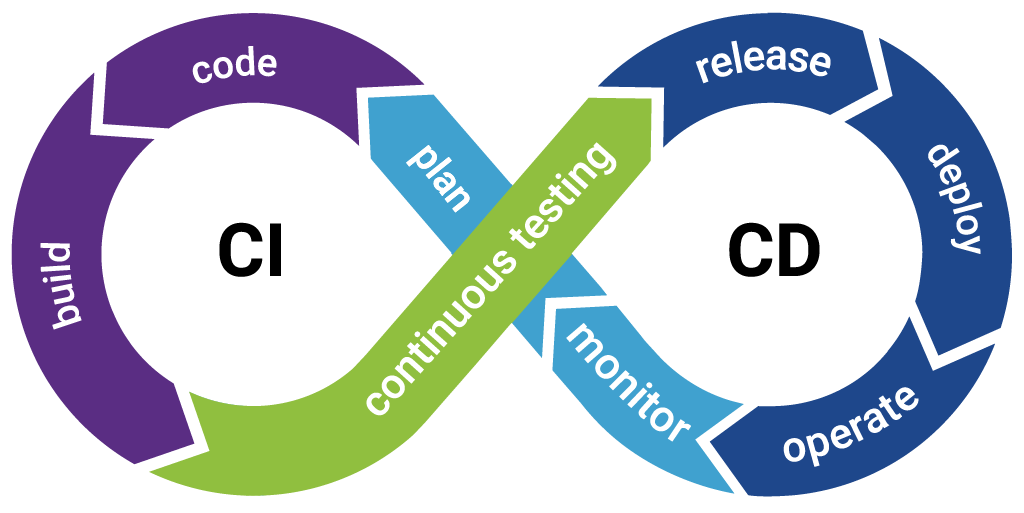
\includegraphics[width=10cm]{ci-cd-diagram}
    \centering
\end{figure}
\subsection{Continuous Integration}
The concept of Continuous Integration was first coined by Grady Booch in 1991, but became mainstream with the rise of eXtreme Programming in 1999. The reference book on the topic is \Citeauthor{Duvall2007}'s ``Continuous Integration: Improving Software Quality and Reducing Risk'' that was published in 2007.

Continuous Integration centers around methods of automating the integration of code changes from various contributors into a single software project is known as continuous integration (CI). It's a fundamental DevOps best practice that enables developers to merge code changes into a single repository regularly, after which builds and tests are executed. Before integration, the new code is checked for correctness using automated tools.
\subsection{Continuous Delivery}
Getting code integrated is not enough, eventually it only provides value in the hands of users so it needs to be deployed and end up in a production environment eventually. Continuous Delivery is the capacity to swiftly and reliably deploy updates of all kinds, such as new features, configuration modifications, bug fixes, and experimentation, into production or to the customer.

In 2010, \Citeauthor{Humble2010} and David Farley published their milestone book ``Continous Delivery, Reliable Software Releases through Build, Test, and Deployment Automation''. This book brings an extended view on process, practices and tools required to get to scalable deployments.

In 2021, \Citeauthor{Farley2021} published a sequel book on the topic titled ``Continuous Delivery Pipelines: How To Build Better Software Faster''. it is a quick read full of practical tips to get started with Continuous Delivery.

The objective is to make deployments predictable, routine tasks that can be carried out on demand, including a large-scale distributed system, a complex production environment, an embedded device, or an app.

All of this is made possible by our commitment to keeping our code deployable, even in the face of everyday modifications made by teams of hundreds or sometimes thousands of developers. As a result, we do away with code freezes and the integration, testing, and hardening phases that typically come after "dev complete".

\begin{figure}[!h]
    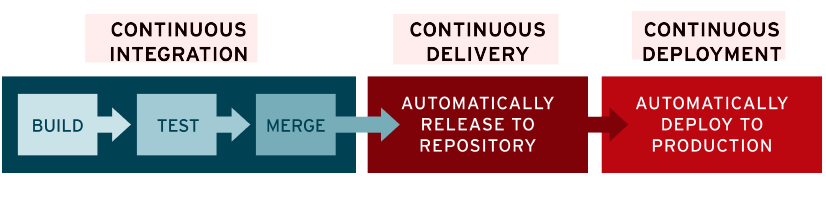
\includegraphics[width=10cm]{ci-cd-flow-desktop_edited_0}
    \centering
\end{figure}
\section{Metrics}
\label{sec:metrics}
Although the project methodology at Showpad centers around \gls{Scrum}, where Velocity is the classic metric to monitor productivity, management uses the traditional lean metrics instead. Before zooming in to the metrics, we set the methodological context in this literature study.
\subsection{Lean Software Development}
There is a lot of literature on measuring team performance and productivity in a software development context. Providing a complete spectrum overview of all methodologies and their related metrics would lead us too far. We focus on the process and its metrics applied at Showpad and will provide the background on these metrics in this literature study.
At Showpad, the core of the metrics set used by management to monitor and control productivity boils down to the lean metrics of \gls{Cycletime}, Throughput, and Work In Progress. 
\newline
\newline
Lean software metrics build on the industrial production methodology called the Toyota Production System. Unlike the design and mass production of physical products, designed by engineers and produced by machines in factories, the design, creation, maintenance, and evolution of software products are fundamentally different, so the usage of lean methodologies and metrics have to be tuned towards this other reality.
\newline
\newline
In their 2007 book ``Implementing Lean Software Development: From Concept to Cash''  \Citeauthor{Poppendieck2007} give an excellent overview of how the lean concepts and practices in manufacturing translate to the world of software development. In Chapter 5 of the book, they zoom in on the theme of speed and time to value, bringing us to the core lean metrics: \gls{Cycletime}, Throughput, and Work In Progress. The mathematical relationship between those three core metrics is illustrated by explaining Little's Law.
\newline
\newline
In his  2018 book ``Project to Product, how to survive and thrive in the age of digital disruption with the flow framework'', \Citeauthor{Kersten2018} builds further on the lean legacy. Based on his analysis of the manufacturing practices observed in the Leipzig BMW plant, he looks for the commonalities and differences between modern lean-based car production processes and procedures and their software development counterparts. In his book, Kersten describes the epiphanies he encountered throughout his research. His 3rd epiphany, ``Software value streams are not linear manufacturing processes but complex collaboration networks that need to be aligned to products'' goes to the fundamental difference between applying lean in the manufacturing context versus the software development context. In a previous section of this chapter, we zoomed in on state of the art on Architectural patterns as they are applied at Showpad. Kersten's first epiphany, ``Software productivity declines and thrashing increases as software scales, due to disconnects between the architecture and the value stream.'' connects the dots and helps understand how architectural choices influence the productivity in a software organization.
\subsection{Lean Metrics and Flow}
Where Poppendieck's and Kersten's books put the lens on the lean software development methodology, another great book zooming into the lean metrics is the book titled  ``Actionable Agile Metrics for Predictability, and introduction'' by \Citeauthor{Vacanti2015}. This book solely focuses on core lean metrics, zooms in on the relationship defined by Little's law, and elaborates on the concept of flow. It also deep dives into continuous flow diagrams to illustrate and analyze flow.
\subsection{Little's Law} 
Little's Law is a queueing theorem by John Dutton Conant Little. The formula is streight forward: \begin{math}L = \lambda * W \end{math}.
Where \begin{math}L \end{math}
 is the average number of items in the queueing system.
 \begin{math} \lambda \end{math}  
 is the average number of items arriving per unit of time. And 
 \begin{math}W \end{math} 
 is the average wait time in the system for 1 item.
\newline
\newline
In the software development context, the ``item'' is a unit of work. As mentioned in the Introduction chapter, in Showpad, there are two granularity levels when thinking about work units. An \gls{Epic} is the top-level units of work, all Epics together composing the Roadmap. Epics are typically delivered in 1 release cycle. An \gls{Epic} is further broken down into several User Stories. A user story is generally delivered in 1 sprint. A user story is the unit of work for one \gls{Scrum} team. So when we want to get a view of the productivity of a \gls{Scrum} team, the Item in Little's Law formula is a user story.
\newline
\newline
In chapter 3 of his book, Vacati translates Little's law to the three lean metrics.
\newline
\newline
Average \gls{Cycletime} = Average Work In Progress / Average Throughput
\newline
\newline
\subsection{Cycle Time}
From a business perspective, the core question \gls{Cycletime} answer is: How long (elapsed time) will the promised work take to complete?
\newline
\newline
\Gls{Cycletime} is the elapsed time from the start of the first task to finishing the last job to deliver 1 item. In the context of a \gls{Userstory}, the clock starts ticking when anyone starts working on the \gls{Userstory} until the last task to deliver the \gls{Userstory} is finished. When evaluating \gls{Cycletime} in the context of an \gls{Epic}, the clock starts ticking when anyone starts working on the first \gls{Userstory} until the last \gls{Userstory} to deliver the \gls{Epic} is finished.
\newline
\newline
Important to mention is that \gls{Cycletime} includes both value-added time (people actively working on tasks) and non-value-added time (waiting time, for example).
\newline
\newline
According to Little's Law: \gls{Cycletime} = Work In Progress / Throughput
\newline
\newline
In the context of Showpad, management talks about Lead Time instead of \gls{Cycletime}. Lead Time and \gls{Cycletime} are two terms that get regularly mixed up. In manufacturing, the distinction is more straightforward. \Gls{Cycletime} covers an individual process step, while Lead Time covers the entire process. As delivering a piece of software takes multiple process steps, even on \gls{Userstory} level, there is the tendency to use the term Lead Time instead of \gls{Cycletime}. As both terms share the same formula but mainly differ on scope level, and for simplicity's sake, we will stick to the usage of \gls{Cycletime} throughout this thesis.
\subsection{Throughput}
From a business perspective, the core question "Throughput" answer is: How many features can I expect?
\newline
Throughput is the ultimate productivity metric. It indicates how many work items we can deliver in a period of time. Translated to the context of Showpad, how many user stories can we deliver in 1 \gls{Sprint}, and how many \glspl{Epic} can we deliver in 1 release cycle.
\newline
\newline
According to Little's Law: Throughput = Work In Progress / \gls{Cycletime}
\newline
\subsection{Work In Progress}
Work In Progress (WIP) equals the number of work items that are worked on in parallel. 
\newline
\newline
Work In Progress does not line up with a direct customer question in business, but it is one of the most influential metrics regarding flow. And limiting Work in Progress is one of the most effective ways to minimize \gls{Cycletime} and maximize Throughput.
\newline
\newline
According to Little's Law: Work In Progress = \gls{Cycletime} * Throughput
